% !TEX root = ../../thesis.tex
%
\chapter{Testing applied to production systems}
\label{sec:testing}

In this chapter, we tackle the problem of testing production
systems, without disturbing them, and without having any
specification \emph{a priori}. Those two constraints sounds
familiar as they have already been taken into consideration in
Chapter \ref{sec:modelinf:prodsystems}. We present a passive
testing technique built on-top of \emph{Autofunk v3}. First, we
infer reference models of a system under analysis $\mathit{Sua}$
using the technique presented previously.  Then, we check whether
a system under test $\mathit{Sut}$ conforms to these inferred
models by means of two implementation relations. We use a
slightly modified version of the trace preorder relation to
strictly check conformance between the two systems. Because the
inferred models are partial, they likely lack information, which
implies that our first strict relation may be too "strong".  That
is why we propose a second (weaker) implementation relation to
comply with Michelin's needs.  Such a relation is less strict
than the first one in order to accept non-standard behaviors down
to a certain point. These two relations are leveraged in an
algorithm for performing offline passive conformance testing.  We
end this chapter with a few results on this testing technique.\\

\minitoc

\pagebreak

\section{Introduction}
\label{sec:testing:intro}

Manual testing is, by far, the most popular technique for
testing, but this technique is known to be error-prone as well.
As already formulated in this thesis, production systems are
usually composed of thousands of states (\emph{i.e.} sets of
conditions that exist at a given instant in time) and production
events, which makes testing time consuming.  In this context, we
propose a \emph{passive testing framework} for production systems
that is compound of: (i) a model inference engine, already
presented in Chapter \ref{sec:modelinf:prodsystems}, and (ii) a
passive test engine, which is the purpose of this chapter. Both
parts have to be fast and scalable to be used in practice.

The main idea of our proposal is that, given a running production
system, for which active testing cannot be applied, we extract
knowledge and models. Such models describe the functional
behaviors of the system, and may serve different purposes,
\emph{e.g.}, testing another production system. The latter can be
a new system roughly comparable to the first one in terms of
features, but it can also be an updated version of the first one.
Indeed, upgrades might inadvertently introduce faults, and it
could lead to severe damages.

In our context, testing the updated system means detecting potential
regressions before deploying changes in production. This is
usually performed by engineers at Michelin, yet their "testing"
phase is actually a manual task performed in a simulation room
where they check a couple of known scenarios for a long period
(about 6 months). Most of the time, such a process works well,
but it takes a lot of time, and there is no guarantee regarding
the number of covered scenarios. In addition, engineers who write
or maintain the applications are likely the same who perform
these manual testing phases, which can be problematic because
they often know too well the applications. We designed our
testing framework to help Michelin engineers focus on possible
failures, automatically highlighted by the framework in a short
amount of time. At the end, engineers still have to perform a few
manual tasks, but they are more efficient as they have only a few
behaviors to check (instead of all possible behaviors), given in
a reliable and fast manner.

Generally speaking, a \textit{passive tester} (also known as
observer) aims at checking whether a system under test
\emph{conforms to} a model. It can be performed in either online
or offline mode, as defined below:

\begin{itemize}
    \item \textbf{Online testing:} it means that traces are
        computed and analyzed on-the-fly to provide verdicts, and
        no trace set is studied \emph{a posteriori};

    \item \textbf{Offline testing:} it means that a set of traces
        has been collected while the system is running. Then, the
        tester gives verdicts afterwards.
\end{itemize}

In this Chapter, we present an offline passive testing technique.
We collect the traces of the system under test by reusing
\textit{Autofunk v3}'s Models generator, and we build a set of
traces whose level of abstraction is the same as those considered
for inferring models. Then, we use these traces to check whether
the system under test conforms to the inferred models.  In
previous works, we used to work with fixed sets of traces. We
noticed that, by taking large trace sets, we could build more
complete models, and performing offline passive testing allows to
use such large trace sets.

\emph{Conformance} is defined with two implementation relations,
which express precisely what the system under test should do. The
first relation is based on the \emph{trace preorder}
\cite{DNH84}, which is a well-known relation based upon trace
inclusion, and heavily used with passive testing.  Nevertheless,
our inferred models are partials, \emph{i.e.} they do not
necessarily capture all the possible behaviors that should
happen. That is why we propose a second implementation relation,
less restrictive on the traces that should be observed from the
system under test.

In Section \ref{sec:testing:normal}, we introduce an extra step
of the model inference method described in Chapter
\ref{sec:modelinf:prodsystems} that is required to enable
testing. In Section \ref{sec:testing:passive}, we present our
offline passive testing technique, built on-top of this model
inference framework. We present key results on offline passive
testing in Section \ref{sec:testing:offline:impl-exp}. Finally,
we conclude on this chapter in Section
\ref{sec:testing:conclusion}.

\textbf{Publication.} This work has been partially published in
the Proceedings of the 13th International Conference on Formal
Methods and Models for Co-Design (MEMOCODE'15) \cite{7340480}.

%%%%%%%%%%%%%%%%%%%%%%%%%%%%%%%%%%%%%%%%%%%%%%%%%%%%%%%%%%%%%%%%%

\section{Normalization of the inferred models}
\label{sec:testing:normal}

In order to perform testing, we reuse the reduced model set
$R(\EuScript{S}) = \{R(\EuScript{S}_1),\dots,R(\EuScript{S}_n)\\
\}$ inferred with \textit{Autofunk} that we \textit{normalize} to
get rid of some runtime-dependent information of the system under
analysis $\mathit{Sua}$. Indeed, both models $\EuScript{S}_i$ and
$R(\EuScript{S}_i)$ include parameters that are dependent to the
products being manufactured. That is a consequence of generating
models that describe behaviors of a continuous stream of products
that are strictly identified. For instance, each action in a
given sequence owns the assignment $(pid := val)$ (for the
record, $pid$ stands for \emph{product identifier}). Collected
traces are also time-dependent, which would make testing of
another production system unfeasible. These information are
typically known by a human domain expert, and we can use
inference rules to identify and remove assignments one more time.

Given the model sets $\EuScript{S} =
\{\EuScript{S}_1,\dots,\EuScript{S}_n\}$ and $R(\EuScript{S}) =
\{R(\EuScript{S}_1),\dots,R(\EuScript{S}_n)\}$, we remove the
assignments related to product identifiers and time stamps to
produce normalized model sets, denoted by $\EuScript{S}^{N} = \{
\EuScript{S}_1^{N}, \dots, \EuScript{S}_n^{N} \}$ and
$R(\EuScript{S}^{N}) = \{ R(\EuScript{S}_1^{N}), \dots,
R(\EuScript{S}_n^{N}) \}$.

Furthermore, we label all the final locations with
"Pass". We flag these locations as \emph{verdict locations}, and
gather them in the set $Pass \subseteq L_{\EuScript{S}_i^{N}}$.
Both $\EuScript{S}_i^{N}$ and $R(\EuScript{S}_i^{N})$ represent more
generic models, \emph{i.e.}  they express \textit{some possible
complete behaviors that should happen}. These behaviors are
represented by the traces $Traces_{Pass}
(\EuScript{S}^{N})=\displaystyle \bigcup_{1 \leq i \leq n}
Traces_{Pass} (\EuScript{S}_i^{N})=Traces_{Pass}
(R(\EuScript{S}^{N}))$. We refer to these traces as \textit{pass
traces}, and we call the other traces \textit{possibly fail
traces}.

%%%%%%%%%%%%%%%%%%%%%%%%%%%%%%%%%%%%%%%%%%%%%%%%%%%%%%%%%%%%%%%%%

\section{Passive testing with \textit{Autofunk}}
\label{sec:testing:passive}

We consider both model sets $\EuScript{S}^{N}$ and
$R(\EuScript{S}^{N})$ of a system under analysis $\mathit{Sua}$,
generated by our inference-based model generation framework, as
\emph{reference models}. In this section, we present the second
part of our testing framework, dedicated to the passive testing
of a system under test $\mathit{Sut}$.

Figure \ref{fig:passive-autofunk} depicts the design of our
offline passive testing technique. A set of production events has
been collected beforehand from $\mathit{Sut}$ in the same way as
for $\mathit{Sua}$. These events are grouped into traces to form
the trace set $Traces({Sut})$, and then filtered to obtain a set
of complete traces denoted by $CTraces({Sut})$ (cf.
\crossref{sec:modelinf:prodsystems}{sec:modelinf:prodsystems:better-segmentation}).
Finally, we perform passive testing to \emph{check} if
$\mathit{Sut}$ conforms to $\EuScript{S}^{N}$.

\begin{figure}[h]
    \begin{center}
        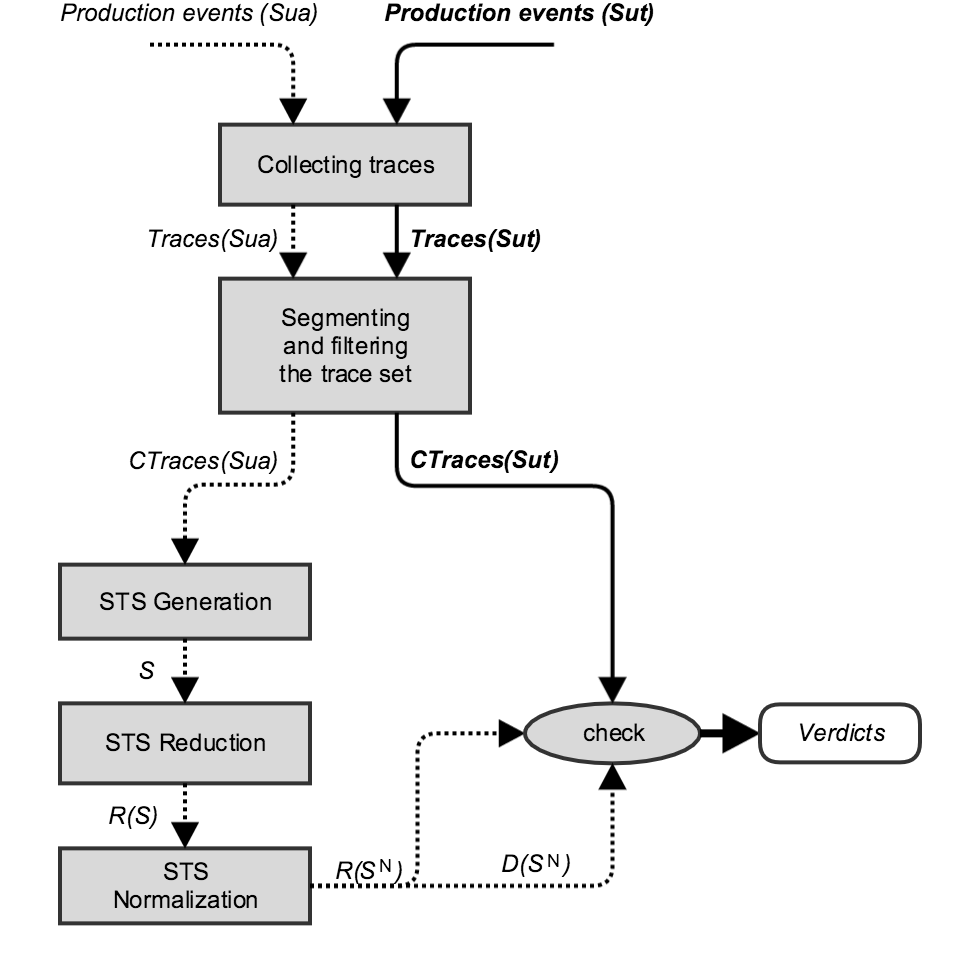
\includegraphics[width=1.0\linewidth]{figures/passive_autofunk.png}
    \end{center}

    \caption{Overview of \textit{Autofunk v3} with the
    passive testing extension. While the previous
    \textit{Autofunk} design has been kept, there are
    two new modules: "STS Normalization" and "check",
    representing the passive conformance testing part.}
    \label{fig:passive-autofunk}
\end{figure}

Our industrial partner wishes to check whether every complete
execution trace of $\mathit{Sut}$ matches a behavior captured by
$\EuScript{S}^{N}$. In this case, the test verdict must reflect a
successful result. On the contrary, if an execution of
$\mathit{Sut}$ is not captured by $\EuScript{S}^{N}$, one cannot
conclude that $\mathit{Sut}$ is faulty because $\EuScript{S}^{N}$
is a partial model, and it does not necessarily includes all the
correct behaviors. Below, we formalize these verdict notions
with two implementation relations. Such relations between models
can only be written by assuming the following \emph{test
assumption}: the black-box system $\mathit{Sut}$ can be described
by a model, here with a Labeled Transition System as defined in
\crossref{sec:related:testing}{sec:definitions:lts}. For
simplicity purpose, we also denote this model by $\mathit{Sut}$.

It is manifest that both the models and $\mathit{Sut}$ must be
\emph{similar}, \emph{i.e.} the production events captured on
$\mathit{Sua}$ and $\mathit{Sut}$ must lead to similar valued
events. Otherwise, all traces of $\mathit{Sut}$ will likely be
rejected, and the testing process will become wasteful:

\begin{definition}[Similarity of $\EuScript{S}^N$ and $\mathit{Sut}$]
    Let $\EuScript{S}^N = \{ \EuScript{S}_1^N, \dots,
    \EuScript{S}_n^N \}$ be a STS set, and $\mathit{Sut}$ be a LTS
    (semantics), which is assumed to behave as the production
    system.

    $\EuScript{S}^N$ and $\mathit{Sut}$ are said \emph{similar}
    if and only if: $\displaystyle\Sigma_{Sut} \subseteq \bigcup_{1 \leq i \leq n}
    \bigcup_{a(p) \in \Lambda_{\EuScript{S}_i^N}} a \times D_p$.

    \label{def:similar-sut-sua}
\end{definition}

\subsection{First implementation relation: $\leq_{ct}$}

The first implementation relation, denoted by $\leq_{ct}$, refers
to the trace preorder relation
\cite{DNH84,vaandrager1991relationship} (cf. Example
\ref{example:trace_preorder} on page
\pageref{example:trace_preorder}).
It aims at checking whether all the complete execution traces of
$\mathit{Sut}$ are pass traces of
$\EuScript{S}^{N}=\{\EuScript{S}_1^{N},\dots,\EuScript{S}_n^{N}\}$.
The first implementation relation can be written with the
following definition:

\begin{definition}[Implementation relation $\leq_{ct}$]
\label{rel:impl1}

Let $\EuScript{S}^{N}$ be an inferred model of $\mathit{Sua}$, and
$\mathit{Sut}$ be the system under test. When $\mathit{Sut}$
produces complete traces also captured by $\EuScript{S}^{N}$, we
write: ${Sut} \leq_{ct} \EuScript{S}^{N} =_{def} CTraces({Sut})
\subseteq  Traces_{Pass}(\EuScript{S}^{N})$.
\end{definition}

Pragmatically, the reduced model set $R(\EuScript{S}^{N})$ sounds
more convenient for passively testing $\mathit{Sut}$ because it
is strongly reduced in terms of size compared to
$\EuScript{S}^{N}$. The test relation can also be written
as below because both models $\EuScript{S}^{N}$ and
$R(\EuScript{S}^{N})$ are trace equivalent (cf. Proposition
\ref{prop:trace-eq-r} in Chapter \ref{sec:modelinf:prodsystems}):

\begin{proposition}
\label{rel:impl12}
${Sut} \leq_{ct} \EuScript{S}^{N} \Leftrightarrow CTraces({Sut})
\subseteq  Traces_{Pass}(R(\EuScript{S}^{N}))$.
\end{proposition}

\subsection{Second implementation relation: $\leq_{mct}$}

As stated previously, the inferred model $\EuScript{S}^{N}$ of
$\mathit{Sua}$ is partial, and it might not capture all the
behaviors that should happen on $\mathit{Sut}$. Consequently,
our partner wants a \emph{weaker implementation relation} that is
less restrictive on the traces that should be observed from
$\mathit{Sut}$. This second relation aims to
check that, for every complete trace $t=(a_1(p), \alpha_1) \dots
(a_m(p), \alpha_m)$ of $\mathit{Sut}$, we also have a set of traces of
$Traces_{Pass}(\EuScript{S}^{N})$ having the same sequence of
symbols such that every variable assignment $\alpha_j(x)_{(1 \leq
j \leq m)}$ of $t$ is found in one of the traces of
$Traces_{Pass}(\EuScript{S}^{N})$ with the same symbol $a_j$.

\begin{example}
    Figure \ref{fig:sts-ch4} recalls the example considered in
    Chapter \ref{sec:modelinf:prodsystems}. The trace $t =
    (17011(\{ nsys, nsec, point, pid \}), \{
    nsys:=1, nsec:=8, point:=1, pid:=1 \})\text{ }
    17021(\{ nsys, nsec, point, tpoint, pid \}, \{
    nsys:=1, nsec:=8, point:=4, tpoint\\:=9, pid:=1 \})$ is not
    a \emph{pass trace} of $\EuScript{S}^{N}$ because this trace
    cannot be extracted from one of the paths of the STS depicted
    in Figure \ref{fig:sts-ch4}, on account of the variables
    $point$ and $tpoint$, which do not take the expected values.
    Nonetheless, both variables are assigned with $(point := 4)$
    and $(tpoint := 9)$ in the second path. This is interesting
    as it indicates that such values \emph{may} be correct since
    they are actually used in a similar action in a similar path.
    Our second implementation relation aims at expressing that
    such a trace $t$ captures a correct behavior as well.

    \begin{figure}[ht]
        \begin{center}
            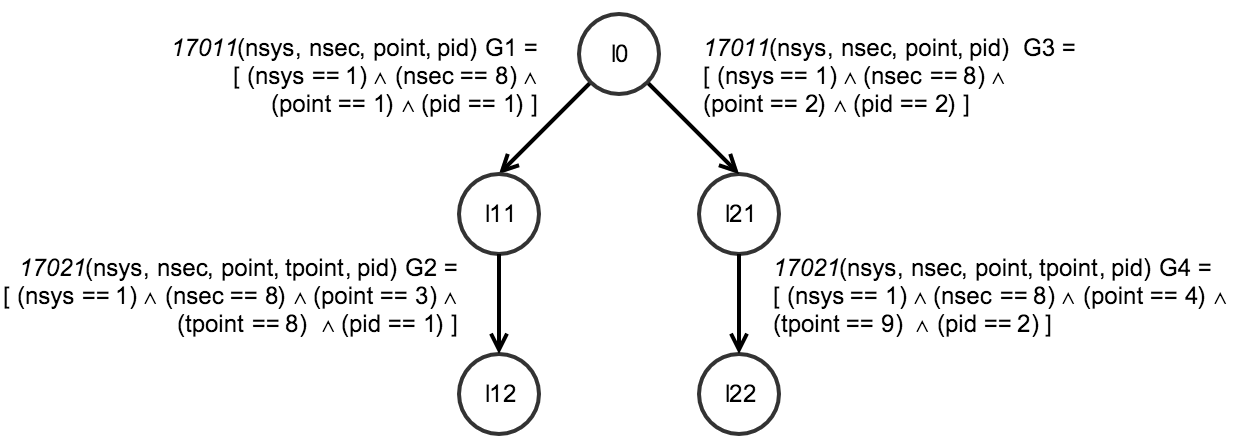
\includegraphics[width=1.0\linewidth]{figures/STS1.png}
        \end{center}

        \caption{The first Symbolic Transition System inferred in
        Chapter \ref{sec:modelinf:prodsystems}.}
        \label{fig:sts-ch4}
    \end{figure}
\end{example}

The second implementation relation, denoted by $\leq_{mct}$, is
defined as follows:

\begin{definition}[Implementation relation $\leq_{mct}$]
     Let $\EuScript{S}^{N}$ be an inferred model of
     $\mathit{Sua}$, and $\mathit{Sut}$ be a system under test.
     We write: ${Sut} \leq_{mct} \EuScript{S}^{N}$ if and only if
     $\forall ~t= (a_1(p), \alpha_1) \dots (a_m(p), \alpha_m) \in
     CTraces({Sut})$, $\forall ~\alpha_j(x)_{(1 \leq j \leq m)},
     \exists ~\EuScript{S}_i^{N} \in \EuScript{S}^{N}$ and $t'
     \in Traces_{Pass}(\EuScript{S}_i^{N})$ such that
     $t'=(a_1(p), \alpha_1') \dots (a_m(p), \alpha_m')$ and
     $\alpha_j'(x)=\alpha_j(x)$.

     \label{impl21}
\end{definition}

According to the above definition, the successive symbols and
variable assignments of a trace $t \in CTraces({Sut})$ can be
found into several traces of $Traces_{Pass}(\EuScript{S}_i^{N})$,
which have the same sequence of symbols $a_1 \dots a_m$ as the
trace $t$. The reduced model $R(\EuScript{S}_i^{N})$ was
previously constructed to capture all these traces in
$Traces_{Pass}(\EuScript{S}_i^{N})$, having the same sequence of
symbols. Indeed, given a STS $\EuScript{S}_i^{N}$, all the STS
paths of $\EuScript{S}_i^{N}$, which have the same sequence of
symbols labeled on the transitions, are packed into one STS path
$b$ in $R(\EuScript{S}_i^{N})$ whose transition guards are stored
into a matrix $M_{[b]}$.

\begin{example}
    Given our trace example $t = (17011(\{ nsys, nsec, point, pid
    \}), \{ nsys\\:=1, nsec:=8, point:=1, pid:=1 \})\text{ }
    17021(\{ nsys, nsec, point, tpoint, pid \}, \{ nsys\\:=1,
    nsec:=8, point:=4, tpoint:=9, pid:=1 \})$, and the reduced
    model depicted in Figure \ref{fig:sts-reduced-ch4}, $t$ is a
    pass trace with respect to $\leq_{mct}$ because each
    assignment $\alpha_j(x)$ satisfies at least one guard of the
    matrix line $j$. For instance, the assignment $(point := 4)$,
    which is given with the second valued event of $t$,
    satisfies one of the guards of the second line of the matrix
    $M_{[b]}$.

    \begin{figure}[h]
        \begin{center}
            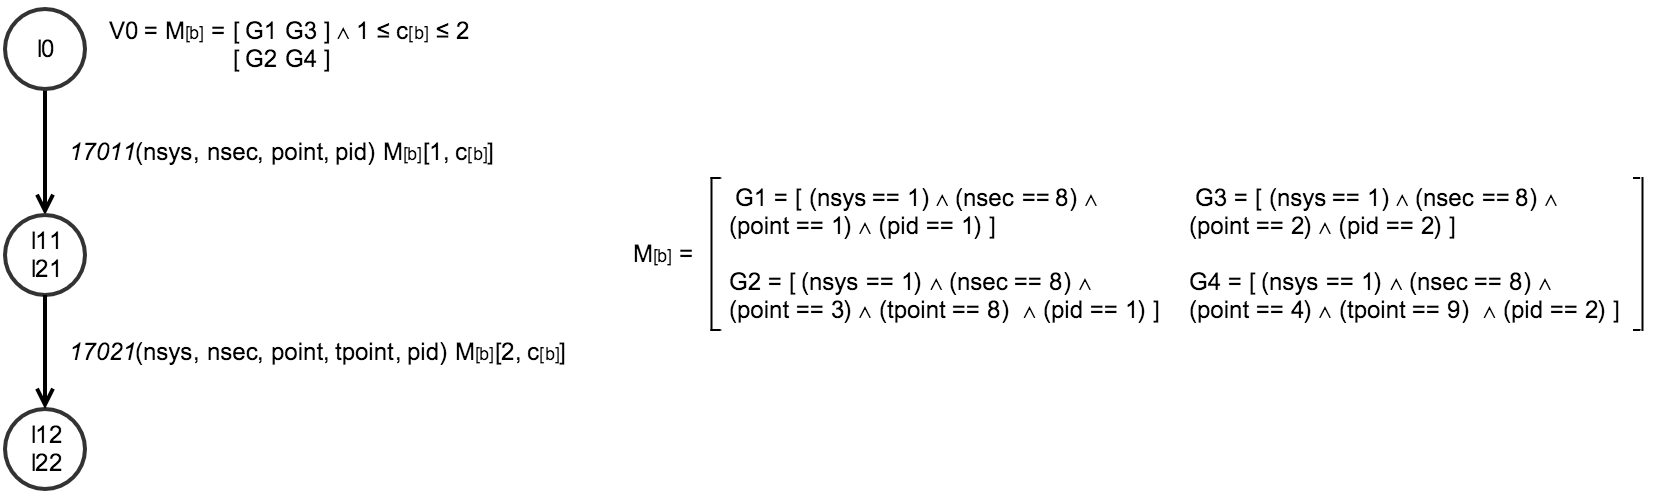
\includegraphics[width=1.0\linewidth]{figures/reduced_sts_ch4.png}
        \end{center}

        \caption{Reduced Symbolic Transition System model (with
        its matrix) obtained from the model depicted in Figure
        \ref{fig:sts-ch4}.}
        \label{fig:sts-reduced-ch4}
    \end{figure}
\end{example}

Given a trace $(a_1(p), \alpha_1) \dots (a_m(p), \alpha_m) \in
CTraces({Sut})$ and a STS path $b$ of $R(\EuScript{S}_i^{N})$
having the same sequence of symbols $a_1 \dots a_m$, the relation
can now be formulated as follows: for every valued event
$(a_j(p), \alpha_j)$, each variable assignment $\alpha_j(x)$ must
satisfies at least one of the guards of the matrix line $j$ in
$M_{[b]}[j,*]$.

Consequently, we propose to rewrite the implementation relation
$\leq_{mct}$ as:

\begin{proposition}
    ${Sut} \leq_{mct} \EuScript{S}^{N}$ if and only if
    $\forall ~t = (a_1(p), \alpha_1) \dots (a_m(p), \alpha_m) \in
    CTraces({Sut})$, $\exists ~R(\EuScript{S}_i^{N}) \in
    R(\EuScript{S}^{N)}$ and
    $b = l0_{R(\EuScript{S}_i^{N})}
    \xRightarrow{(a_1(p_1),M_{[b]}[1,c_{[b]}]) \dots (a_j(p_j),M_{[b]}[j,c_{[b]}])}
    l_m$
    with $(1 \leq c_{[b]} \leq k)$ such that $\forall
    ~\alpha_j(x)_{(1 \leq j \leq m)}, \alpha_j(x) \models
    M_{[b]}[j,1] \vee \dots \vee  M_{[b]}[j,k]$, and $l_m \in Pass$.
\end{proposition}

The disjunction of guards $M_{[b]}[j,1] \vee \dots \vee
M_{[b]}[j,k]$, found in the matrix $M_{[b]}$, could be simplified
by gathering all the equalities $(x == val)$ together with
disjunctions for every variable $x$ that belongs to the parameter
set $p_j$ of $a_j(p_j)$. Such equalities can be extracted with
the projection operator \textit{proj} (see Definition
\ref{def:sts}). We obtain one guard of the form $\displaystyle
\bigwedge_{x \in p_j} ((x == val_1) \vee \dots \vee (x ==
val_k))$. This can be expressed by deriving new STSs from
$R(\EuScript{S})$.

\subsection{STS $D(\EuScript{S})$}

Given a STS $R(\EuScript{S}_i^{N})$, the STS
$D(\EuScript{S}_i^{N})$ is constructed with the disjunction of
guards described in the previous section:

\begin{definition}[Derived STS $D(\EuScript{S}_i^{N})$]
    Let
    $R(\EuScript{S}_i^{N})=<L_R,l0_R,V_R,V0_R,I_R,\Lambda_R,\rightarrow_R>$
    be a STS of $R(\EuScript{S}^{N})$. We denote by
    $D(\EuScript{S}_i^{N})$ the STS $
    <L_D,l0_D,V_D,V0_D,I_D,\Lambda_D,\rightarrow_D>$ derived from
    $R(\EuScript{S}_i^{N})$ such that:

    \begin{itemize}
        \item $L_D=L_{R}$;

        \item $l0_D=l0_{R}$;

        \item $I_D=I_{R}$;

        \item $\Lambda_D=\Lambda_{R}$;

        \item $V_D, V0_D$ and $\rightarrow_D$ are defined by the
            following inference rule:

            $\frac{
                \begin{matrix}
                b=l0_{R}
                \xRightarrow{(a_1(p_1),M_{[b]}[1,c_{[b]}])\dots
                (a_m(p_m),M_{[b]}[m,c_{[b]}])}_{R}
                l_{m},
                (1 \leq c_{[b]} \leq k) \text{ in } V0_{R}
                \end{matrix}
            }
            {
                \begin{matrix}
                l0_D
                \xRightarrow{(a_1(p_1),M_{b}[1])\dots (a_m(p_m),M_{b}[m])}_{D}
                l_m, V0_D=V0_D \wedge M_{b},\\
                M_{b}[j]_{(1\leq j \leq m)} = \displaystyle
                \bigwedge_{x \in p_j} ( proj_x(M_{[b]}[j, 1])
                \vee \dots \vee proj_x(M_{[b]}[j, k]))

                \end{matrix}
            }$
    \end{itemize}

    The set of derived models is denoted by $D(\EuScript{S}^{N}) =
    \{D(\EuScript{S}_1^{N}),\dots,D(\EuScript{S}_n^{N}) \}$.

    \label{def:sts-d}
\end{definition}

The second implementation relation $\leq_{mct}$ can now be
expressed by:

\begin{proposition}
    ${Sut} \leq_{mct} \EuScript{S}^{N}$ if and only if $\forall
    ~t= (a_1(p), \alpha_1) \dots (a_m(p), \alpha_m) \in CTraces({Sut})$,
    $\exists ~D(\EuScript{S}_i^{N}) \in D(\EuScript{S}^{N})$ and
    $l0_{D(\EuScript{S}_i^{N})} \xRightarrow{(a_1(p_1),G_{1})
    \dots (a_m(p_m),G_{m})} l_m$ such that $\forall
    ~\alpha_{j ~(1 \leq j \leq m)}, \alpha_j \models G_{j}$ and
    $l_m \in Pass$.
\end{proposition}

The implementation relation $\leq_{mct}$ now means that a trace
of $\mathit{Sut}$ must also be a pass trace of the model set
$D(\EuScript{S}^{N})=\{D(\EuScript{S}_1^{N}),\dots,D(\EuScript{S}_n^{N})\}$.
This notion of trace inclusion can also be formulated with the
first implementation relation $\leq_{ct}$ as follows:

\begin{proposition}
    ${Sut} \leq_{mct} \EuScript{S}^{N} \text{ if and only if }
    CTraces({Sut})\subseteq
    Traces_{Pass}(D(\EuScript{S}^{N}))$, and ${Sut} \leq_{mct}
    \EuScript{S}^{N} \Leftrightarrow {Sut} \leq_{ct}
    D(\EuScript{S}^{N})$.

    \label{rel:impl2}
\end{proposition}

Now, the implementation relation $\leq_{mct}$ is expressed with
the first relation $\leq_{ct}$, which implies that our passive
testing algorithms shall be the same for both relations except
that they shall take different reference models.

Furthermore, because $D(\EuScript{S}^{N})$ is derived from
$R(\EuScript{S}^{N})$, \emph{i.e.} the guards of the model
$D(\EuScript{S}_i^{N})$ are the disjunctions of the guards of the
model $R(\EuScript{S}_i^{N})$ (cf. Definition \ref{def:sts-d}),
we have $Traces_{Pass}(R(\EuScript{S}^{N})) \subseteq
Traces_{Pass}(D(\EuScript{S}^{N}))$. Therefore, if $\mathit{Sut}
\leq_{ct} \EuScript{S}^N$, we have $\mathit{Sut} \leq_{mct}
\EuScript{S}^N$:

\begin{proposition}
    $\mathit{Sut} \leq_{ct} \EuScript{S}^N \implies
    \mathit{Sut} \leq_{mct} \EuScript{S}^N$.

    \label{rel:impl-ct-implies-mct}
\end{proposition}

In the next section, we introduce the offline passive testing
algorithm that uses these two implementation relations.

\subsection{Offline passive testing algorithm}
\label{sec:testing:offline}

Our offline passive testing algorithm, which aims to check
whether the two previous implementation relations hold, is given
in Algorithm \ref{algo:check}. It takes the complete traces of
$\mathit{Sut}$, as well as the model sets $R(\EuScript{S}^{N})$ and
$D(\EuScript{S}^{N})$, with regard to Proposition
\ref{rel:impl12} and Proposition \ref{rel:impl2}. It returns the
verdict "Pass$\leq_{ct}$" if the relation $\leq_{ct}$ is
satisfied, and the verdict "Pass$\leq_{mct}$" if $\leq_{mct}$ is
satisfied.

Algorithm \ref{algo:check} relies upon the function ${check(Trace
~trace, STS ~\EuScript{S})}$ to check whether the trace $trace =
(a_1(p), \alpha_1) \dots (a_m(p), \alpha_m)$ is a trace of
$\EuScript{S}$. If a STS path $b$ is composed of the same
sequence of symbols than $trace$ (line
\ref{algo:check:line:exists}), the function tries to find a
matrix column (\emph{i.e.} a vector) $M = M_{[b]}[*,c_{[b]}]$ ($1
\leq c_{[b]} \leq k$) such that every variable assignment
$\alpha_j$ satisfies the guard $M[j]$. If such a column of guards
exists, the function returns $True$, and $False$ otherwise (cf.
Proposition \ref{prop:check}).

First, this algorithm covers every trace $trace$ of
$CTraces({Sut})$, and tries to find a STS $R(\EuScript{S}_i^{N})$
such that $trace$ is also a trace of $R(\EuScript{S}_i^{N})$ with
$check(trace, R(\EuScript{S}_i^{N}))$ (line
\ref{algo:check:line:check1}).  If no model
$R(\EuScript{S}_i^{N})$ is found, $trace$ is added to the set
$T_1$ (line \ref{algo:check:line:t1}), which gathers the possibly
fail traces with respect to $\leq_{ct}$.
Thereafter, this algorithm performs the same step but using the
STS $D(\EuScript{S}^{N})$ (line \ref{algo:check:line:check2}).
One more time, if no model $D(\EuScript{S}_i^{N})$ is found, the
trace $trace$ is added to the set $T_2$ (line
\ref{algo:check:line:t2}), which gathers the possibly fail
traces with respect to the relation $\leq_{mct}$.
Finally, if $T_1$ is empty, the verdict "Pass$\leq_{ct}$" is
returned, which means that the first implementation relation
holds. Otherwise, $T_1$ is provided. If $T_2$ is empty, the
verdict "Pass$\leq_{mct}$" is returned. Otherwise $T_2$ is
returned.

\begin{algorithm}[h]
    \SetKwInOut{Input}{Input}
    \SetKwInOut{Output}{Output}
    \SetKwFunction{check}{check}

    \Input{
        $R(\EuScript{S}^{N}),
        D(\EuScript{S}^{N}),
        CTraces({Sut})$
    }
    \Output{Verdicts and/or possibly fail trace sets $T_1, T_2$ }

    BEGIN\;

    $T_1 = \emptyset$\;
    $T_2 = \emptyset$\;

    \ForEach{$trace \in CTraces({Sut})$}{

        \For{$i = 1, \dots, n$}{\label{algo:check:line:proof1-start}
            \If{\check($trace$, $R(\EuScript{S}_i^{N})$)}{\label{algo:check:line:check1}
                break\;
            }
        }\label{algo:check:line:proof1-end}

        \If{$i == n$} {
            $T_1=T_1 \cup \{trace\}$\;\label{algo:check:line:t1}

            \For{$i = 1, \dots, n$}{\label{algo:check:line:proof2-start}

                \If{\check($trace$, $D(\EuScript{S}_i^{N})$)}{\label{algo:check:line:check2}
                    break\;
                }
            }\label{algo:check:line:proof2-end}

            \If{$i==n$} {
                $T_2=T_2 \cup \{trace\}$\;\label{algo:check:line:t2}
            }
        }
    }%endfor1

    \BlankLine

    \If{$T_1==\emptyset$}{\label{algo:check:line:empty-t1}
        return "Pass$\leq_{ct}$"\;\label{algo:check:line:pass_ct}
    }
    \Else{
        \If{$T_2==\emptyset$}{\label{algo:check:line:empty-t2}
            return "Pass$\leq_{mct}$" and $T_1$\;\label{algo:check:line:pass_mct}
        }
        \Else{
            return $T_1$ and $T_2$\;
        }
    }

    END\;

    \BlankLine
    \BlankLine

    \SetKwProg{Fn}{Function}{ is}{end}
    \Fn{check(Trace $trace$, STS $\EuScript{S}$) : boolean}{
        \If{$\exists ~b=l0_{\EuScript{S}}
            \xRightarrow{(a_1(p_1),G_{1},A_{1}) \dots
            (a_n(p_n),G_{n},A_{n})} l_n \mid trace =
            (a_1(p), \alpha_1)\dots (a_n(p), \alpha_n)$ and $l_n \in
            Pass$}{\label{algo:check:line:exists}

                $M_{[b]} = Mat(b)$ is the matrix $n \times k$ of $b$\;
                $c_{[b]} = 1$\;
                \While{$c_{[b]} \leq k$}{
                    $M = M_{[b]}[*,c_{[b]}]$\;

                    \For{$j = 1, \dots, n$}{
                        \If{$\alpha_j \not\models M[j]$}{
                            break\;
                        }
                    }

                    \If{$j == n$}{
                        return $True$\;
                    }
                    $c_{[b]}++$\;
                }
        }
        return $False$\;
    }

    \caption{Offline passive testing algorithm}
    \label{algo:check}
\end{algorithm}

When one of the implementation relations does not hold, this
algorithm offers the advantage of providing the possibly fail
traces of $CTraces({Sut})$. Such traces can be later analyzed to
check if $\mathit{Sut}$ is correct or not. That is very helpful
for Michelin engineers because it allows them to only focus on
what are potentially faulty behaviors, reducing debugging time,
and making engineers more efficient.

\begin{proposition}
    Let $t \in CTraces(Sut)$ be a trace, and $\EuScript{S}^{N}$ a
    STS set such that $\mathit{Sut} \leq_{ct} \EuScript{S}^{N}$.
    $\leq_{ct}$ means that there exists a model
    $\EuScript{S}_i^{N}$ such that $t \in
    Traces_{Pass}(\EuScript{S}_i^{N})$, \emph{i.e.} $t$
    \emph{conforms to} $\EuScript{S}_i^{N}$.

    The $check(Trace ~trace, STS ~\EuScript{S})$ function in
    Algorithm \ref{algo:check} implements this relation, and we
    have: $t \in Traces_{Pass}(\EuScript{S}_i^{N}) \implies$ the
    function $check(t, \EuScript{S}_i^{N})$ returns $True$.

    \begin{proof}
        \textbf{Sketch of proof:} Let $t = (a_1(p), \alpha_1)
        \dots (a_n(p), \alpha_n)$ be a trace of $\mathit{Sut}$.
        Let $b$ be a STS path such that
        $\exists ~b=l0_{\EuScript{S}_i^{N}} \xRightarrow{(a_1(p_1),G_{1},A_{1}) \dots
        (a_n(p_n),G_{n},A_{n})} l_n, ~l_n \in Pass \mid ~t \in Traces_{Pass}(b)$.
        Let $M_{[b]}$ be the matrix $n \times k$ of $b$ such that
        $G_j = M_{[b]}[j, c_{[b]}] ~(1 \leq c_{[b]} \leq k)$.

        $Traces_{Pass}(b) = (a_1(p), \beta_1) \dots (a_n(p), \beta_n)$
        with $\beta_1 \dots \beta_n$ such that $\exists ~1 \leq
        c_{[b]} \leq k \mid \beta_j \models G_j ~(1 \leq j \leq n)$.

        Given the trace $t = (a_1(p), \alpha_1) \dots (a_n(p),
        \alpha_n)$, the function $check$:

        \begin{itemize}
            \item finds a path $b = l0_{\EuScript{S}_i^{N}}
                \xRightarrow{(a_1(p_1),G_{1},A_{1}) \dots
                (a_n(p_n),G_{n},A_{n})} l_n, ~l_n \in Pass$ (line
                \ref{algo:check:line:exists});

            \item ensures that $\exists ~1 \leq c_{[b]} \leq k
                \mid \alpha_j \models M_{[b]}[j, c_{[b]}] ~(1
                \leq j \leq n)$ (lines 28-31). %TODO: fixme
        \end{itemize}

        If both a path $b$ and a column $c_{[b]}$ of $M_{[b]}$
        are found, $True$ is returned (line 33).
    \end{proof}

    \label{prop:check}
\end{proposition}

\paragraph{Soundness.} The soundness of Algorithm
\ref{algo:check} can be split into three points (sketch of proof):

\begin{enumerate}
    \item $\mathit{Sut} \leq_{ct} \EuScript{S}^N$ $\implies$
        Algorithm \ref{algo:check} returns "Pass$\leq_{ct}$":

        \begin{proof}
            $\mathit{Sut} \leq_{ct} \EuScript{S}^{N}
            \Leftrightarrow CTraces(Sut) \subseteq Traces_{Pass}(R(\EuScript{S}^N))$
            (Proposition \ref{rel:impl12}) can be written as
            follows: $\forall ~t \in CTraces(Sut), \exists ~1
            \leq i \leq n \mid ~t \in Traces_{Pass}(R(\EuScript{S}_i^{N}))$.

            Given that, and according to Proposition
            \ref{prop:check}, function $check$ returns $True$ for
            every trace $t \in CTraces(Sut)$ (lines
            \ref{algo:check:line:proof1-start}-\ref{algo:check:line:proof1-end}).

            Therefore the set $T_1$ is empty (line
            \ref{algo:check:line:empty-t1}), and Algorithm
            \ref{algo:check} returns "Pass$\leq_{ct}$" (line
            \ref{algo:check:line:pass_ct}).
        \end{proof}

    \item $\mathit{Sut} \leq_{mct} \EuScript{S}^N$ $\implies$
        Algorithm \ref{algo:check} returns "Pass$\leq_{mct}$":

        \begin{proof}
            $\mathit{Sut} \leq_{mct} \EuScript{S}^{N}
            \Leftrightarrow CTraces(Sut) \subseteq Traces_{Pass}(D(\EuScript{S}^N))$
            (Proposition \ref{rel:impl2}) can be written as
            follows: $\forall ~t \in CTraces(Sut), \exists ~1
            \leq i \leq n \mid ~t \in Traces_{Pass}(D(\EuScript{S}_i^{N}))$.

            Given that, and according to Proposition
            \ref{prop:check}, function $check$ returns $True$ for
            every trace $t \in CTraces(Sut)$ (lines
            \ref{algo:check:line:proof2-start}-\ref{algo:check:line:proof2-end}).

            Therefore the set $T_2$ is empty
            (line \ref{algo:check:line:empty-t2}), and Algorithm
            \ref{algo:check} returns "Pass$\leq_{mct}$" (line
            \ref{algo:check:line:pass_mct}).
        \end{proof}

    \item $\mathit{Sut} \leq_{ct} \EuScript{S}^N$ $\implies$
        Algorithm \ref{algo:check} returns "Pass$\leq_{ct}$",
        "Pass$\leq_{mct}$":

        \begin{proof}
            $\mathit{Sut} \leq_{ct} \EuScript{S}^{N} \implies
            \mathit{Sut} \leq_{mct} \EuScript{S}^{N}$
            (Proposition \ref{rel:impl-ct-implies-mct}), therefore
            Algorithm \ref{algo:check} returns "Pass$\leq{ct}$",
            "Pass$\leq_{mct}$".
        \end{proof}
\end{enumerate}

\paragraph{Complexity.}
The complexity of the function $check(t, \EuScript{S})$ is
$\mathcal{O}(m \times k)$ with $m$ the number of valued events in
the trace $t$ (\emph{i.e.} its length), and $k$ the number of
columns in $M_{[b]}$, which is likely large as reduced models
still express all complete behaviors found in the traces of a
system under analysis. Finding a branch in a model is negligible
thanks to the hash mechanism, hence we only take the matrix
traversal into account. Because $m << k$, the complexity of the
function $check(t, \EuScript{S})$ can be simplified to
$\mathcal{O}(k)$.

The complexity of Algorithm \ref{algo:check} is $\mathcal{O}(t
\times n \times k)$ with $t$ the number of complete traces of
$\mathit{Sut}$, $n$ the number of models, and $k$ the complexity
of the $check$ function, which corresponds to the number of
columns of the matrix associated with the branch (as described
above). Compared to the number of traces and columns, the number
of models $n$ is negligible (\emph{i.e.} $n << t$, $n << k$, and
$t \approx k$), which means that the overall complexity is
$\mathcal{O}(t^2)$.

\clearpage

\section{Implementation and experimentation}
\label{sec:testing:offline:impl-exp}

In this section, we summarize the work done on the different
\emph{Autofunk} implementations for Michelin. Then, we give a few
results on our offline passive testing technique.

\subsection{Implementation}

By adding a testing module to \emph{Autofunk v3}, we have
developed a complete tool for testing production systems at
Michelin.

According to the \emph{cloc}
tool\footnote{\url{https://github.com/AlDanial/cloc}}, the latest
version of \emph{Autofunk} has 2831 lines of code written in Java
8, along with 4 Drools rules used in Layer 1 of the model
inference module.  According to
\emph{JaCoCo}\footnote{\url{https://github.com/jacoco/jacoco}}
(which stands for Java Code Coverage) tool, the test suite
(compound of 120 test cases) covers 85\% of the code, with both
unit and functional tests. Our algorithms are extensively tested.

Users of \emph{Autofunk v3} interact with it using the command
line. We designed parallelizable algorithms that we have used in
combination with Java 8 streams and parallel processing
abilities. This gives interesting performance results on
multi-core processors, without affecting code readability.
\emph{Autofunk v3} still embeds Drools, and can either run a
local Spark instance or connect to a Spark cluster, which is
better for performance.  Models are persisted on disk using the
\emph{Kryo}\footnote{\url{https://github.com/EsotericSoftware/kryo}}
serialization library. Finally, this tool is highly configurable
thanks to the (Typesafe)
\emph{Config}\footnote{\url{https://github.com/typesafehub/config}}
library.

Table \ref{fig:autofunk-versions} presents the differences
across all \emph{Autofunk} versions. All versions use Drools to
perform model inference, but only \emph{Autofunk v3} can perform
testing as explained in this chapter. \emph{Autofunk v1} does not
segment the trace set because it is primarily used for web
applications, for which this task does not apply. \emph{Autofunk
v3} is heavily based on \emph{Autofunk v2}, hence both use a
context-specific reduction technique by means of branch
equivalence classes. Yet, \emph{Autofunk v3} uses MLlib for its
k-means implementation, and is more extensively tested.

\begin{sidewaystable}
\begin{center}
    \begin{tabular}{| c | c | c | c | c | c | c |}
        \hline
        \emph{Autofunk} & Use Drools? & Perform inference? & Perform testing? & Segmentation algorithm & Reduction algorithm & Code coverage\\
        \hline
        \hline
        v1 & $\checkmark$ & $\checkmark$ & $\times$ & None & Bisimulation minimization & <50\%\\
        \hline
        v2 & $\checkmark$ & $\checkmark$ & $\times$ & Statistical analysis & Branch equivalence classes & 70\%\\
        \hline
        v3 & $\checkmark$ & $\checkmark$ & $\checkmark$ & K-means (Spark / MLlib) & Branch equivalence classes & 85\%\\
        \hline
    \end{tabular}
\end{center}

    \caption{Summary of the different \emph{Autofunk} versions.
    \emph{Autofunk v3} is based on \emph{Autofunk v2}, which
    has been developed from scratch (even though inspired by
    \emph{Autofunk v1}).}

    \label{fig:autofunk-versions}
\end{sidewaystable}

\subsection{Experimentation}

We conducted several experiments with real sets of production
events, recorded in one of Michelin's factories at different
periods of time. The results given in this section are focused on
our offline passive testing technique, built on-top of
\emph{Autofunk v3}. We executed our implementation on a Linux
(Debian) machine with 12 Intel(R) Xeon(R) CPU X5660 @ 2.8GHz and
64GB RAM.

Table \ref{fig:testing:offline:results} shows the results of
three experiments on the same production system with different
trace sets, recorded at different periods of time, with the
latest \emph{Autofunk} version. The first column shows the
experiment number (\#), columns 2 and 3 respectively give the
sizes of the trace sets of the system under analysis
$\mathit{Sua}$ and of the system under test $\mathit{Sut}$. The
two next columns show the percentage of pass traces with respect
to the relations $\leq_{ct}$ and $\leq_{mct}$. The last column
indicates the execution time (in minutes) for the testing phase.

\begin{table}[h]
\begin{center}
    \begin{tabular}{| c | c | c | c | c | c |}
        \hline
        \# & $Card(CTraces({Sua}))$ & $Card(CTraces({Sut}))$ & Pass$\leq_{ct}$ & Pass$\leq_{mct}$ & Time\\
        \hline
        \hline
        $1$ & 2,075 & 2,075 & 100\% & 100\% & 1 \\
        \hline
        $2$ & 53,996 & 2,075 & 3\% & 30\% & 4\\
        \hline
        $3$ & 53,996 & 25,047 & 98\% & 98\% & 10\\
        \hline
    \end{tabular}
\end{center}

    \caption{This table shows the results of our offline passive
    testing method based on a same specification.}
    \label{fig:testing:offline:results}
\end{table}

In Experiment $1$, we decided to use the same production events
for both inferring models, \emph{i.e.} specifications, and
testing. This experiment shows that our implementation behaves
correctly when trace sets are similar, \emph{i.e.} when behaviors
of both $\mathit{Sua}$ and $\mathit{Sut}$ are equivalent.

Experiment $2$ has been run with traces of $\mathit{Sut}$ that
are older than those of $\mathit{Sua}$, which is unusual as the
\emph{de facto} usage of our framework is to build specifications from a
production system $\mathit{Sua}$, and to take a newer or updated
system as $\mathit{Sut}$.  Here, only 30\% of the traces of
$\mathit{Sut}$ are pass traces with respect to the second
implementation relation (same sequence of symbols with different
values). There are two explanations: (i) the system has been
updated between the two periods of record (4 months), and (ii)
production campaigns, \emph{i.e.} grouping of planned orders and
process orders to produce a certain amount of products over a
certain period of time, were different (revealed by
\textit{Autofunk}, indicating that values for some key parameters
were unknown).

Finally, experiment $3$ shows good results as the specification
models are rich enough, \emph{i.e.}  built from a larger set of
traces (10 days) than the one collected on $\mathit{Sut}$. Such
an experiment is a typical usage of our framework at Michelin.
The traces of $\mathit{Sut}$ have been collected for 5 days, and
it took only 10 minutes to check conformance. While 98\% of the
traces are pass traces, the remaining 2\% (about 500 traces) are
new behaviors that never occurred before. Such a piece of
information is essential for Michelin engineers to detect
potential regressions. Even though 2\% may represent a large set
to analyze (about 500 traces in this experiment),
\textit{Autofunk} eases the work of Michelin engineers by
highlighting the traces to focus on. Instead of having to check
25,000 traces manually, they only have to check 500 traces, which
is a significant improvement on a daily basis.
Yet, such a subset may contain false positives depending on the
richness of the models, but using large sets of traces to infer
the models usually reduces the number of false positives.

\section{Conclusion}
\label{sec:testing:conclusion}

In this chapter, we presented a fast passive testing framework
built on-top of our model inference framework \emph{Autofunk v3},
which combines different techniques such as model inference,
expert systems, and machine learning.

Given a large set of production events, our framework infers
exact models whose traces are included \cite{petrenko06} in the
initial trace set of a system under analysis. Such models are
then reused as specifications to perform: (i) offline passive
testing using a second set of traces recorded on a system under
test, and (ii) online passive testing by taking new traces of a
system under test on-the-fly. Using two implementation relations,
\textit{Autofunk} is able to determine what has changed between
the two systems. This is particularly useful for our industrial
partner Michelin because potential regressions can be detected
while deploying changes in production. Initial results on the
offline method are encouraging, and Michelin engineers see a real
potential in this framework.

We know that 2\% of a large trace set (as mentioned in the
previous section) still represents many traces, which may be
difficult to analyze. Nonetheless in a manufacturing context,
this is still valuable although we would like to reduce such
false negatives.

In the next chapter, we give our thoughts on how to improve
\textit{Autofunk} as well as perspectives for future work.


\cleardoublepage
\blankpage
